\section{Теория множеств}

\subsection{Основные тождества про теоретико-множественные операции, декартово произведение, возведение множества в степень множества}
\begin{itemize}
    \item Коммутативность: $\vee, \wedge, \triangle$
    \item Ассоциативность: $\vee, \wedge, \triangle$
    \item Дистрибутивность: $ \\ A \vee (B \wedge C) = (A \vee B) \wedge (A \vee C) \\ A \wedge (B \vee C) = (A \wedge B) \vee (A \wedge C)$
    \item Идемпотентность: $A \vee A = A, A\wedge A = A$
    \item Аннигиляция: $A \triangle A = \o, A \backslash A = \o$
    \item Законы де Моргана
\end{itemize}
\textbf{Опр} Декартовой степенью множества А называется множество $A^n$: кортеж длины n элементов А
\\
\\
\textbf{Cвойства}
\begin{itemize}
    \item [1] $A^n = A\times A... \times A$ - по определению
     \item [2] $A^{n+k} = \underbrace{A\times A... \times A}_{n}\underbrace{A\times A... \times A}_{k} = \underbrace{A\times A... \times A}_{n+k} = A^n \times A^k$ 
     \item [3] $A\times B)\times C = A \times( B \times C )$\\
     $A \times B = \{(a,b): \ a \in A, b\in B\} \\ (A \times B ) \times C = \{((a,b),c): \ a \in A, b\in B, c \in C\} = \{(a,(b,c)): \ a \in A, b\in B, c \in C\} = A\times (B \times C)$
     \item[4] $A\times (B \vee C) = (A \times B) \vee (A \times C)$ \\ $A \times(B \vee C) = \{ (a,k): \ a \in A, k \in B \ or\ k\in C\} =  \{ (a,k): \ a \in A, k \in B \} $или$\{ (a,k): \ a \in A,\ k\in C\} = (A \times B) \vee (A \times C) $
\end{itemize}

\subsection{Равномощность — отношение эквивалентности.}
\begin{itemize}
    \item [1] $A \cong A$ - биекция - id
    \item [2] $A  \cong B \Longrightarrow B \cong A$ - очевидно
    \item[3]  $A \cong B, B \cong C$ - композиция биекций - биекция, значит $A \cong C$
\end{itemize}

\subsection{Объединение и декартово произведение счётных множеств счётны.}
\begin{center}
    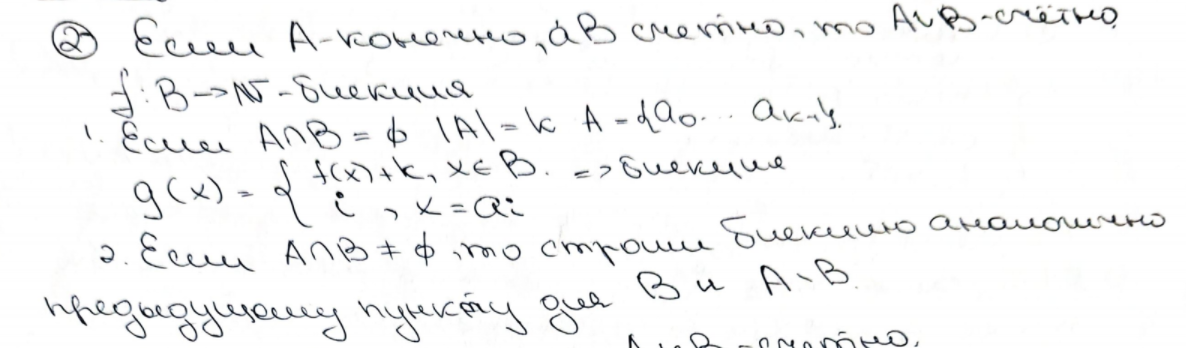
\includegraphics[width = 0.8\textwidth]{images/2 (определения)_m28.PNG}
    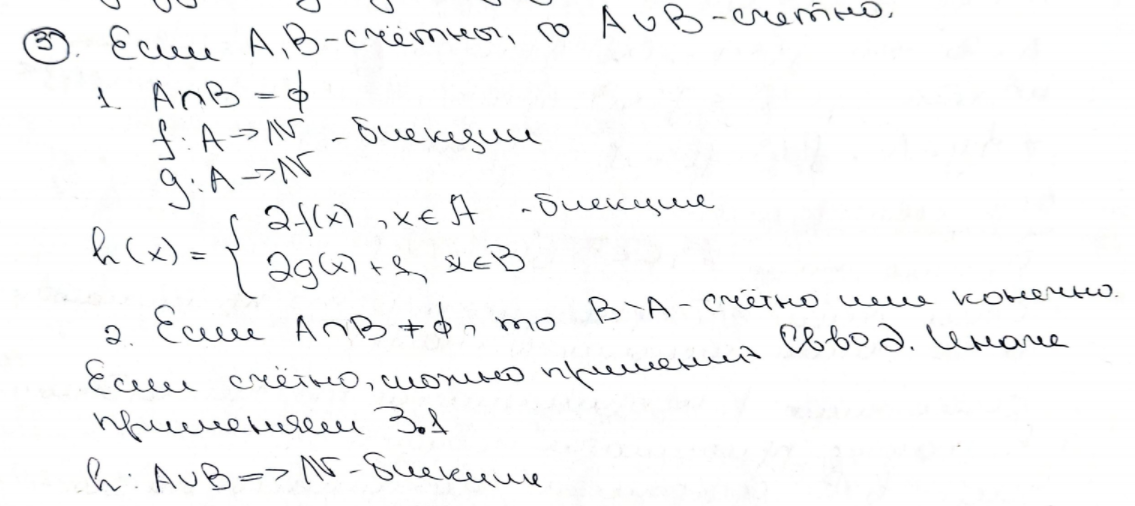
\includegraphics[width = 0.8\textwidth]{images/2 (определения)_m29.PNG}
    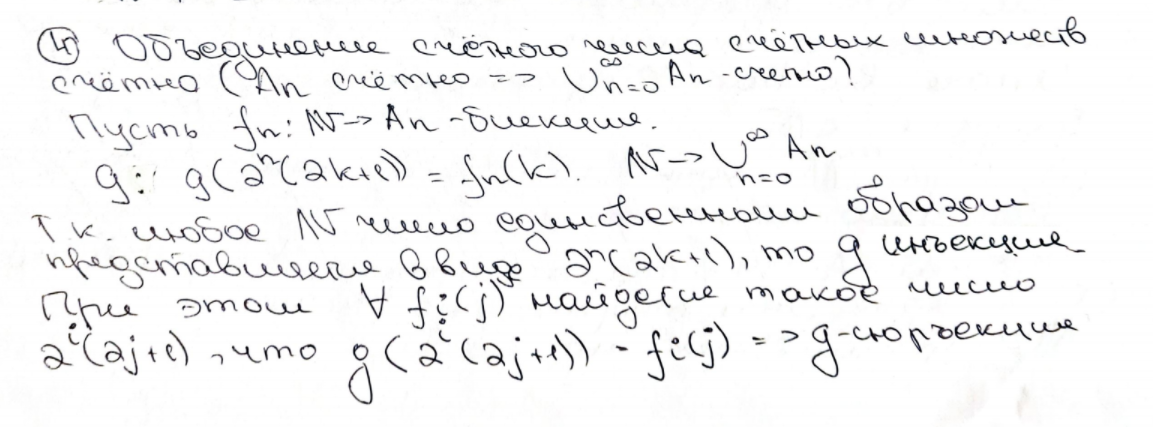
\includegraphics[width = 0.8\textwidth]{images/2 (определения)_m210.PNG}
\end{center}
    
Декартово произведение - это счетное объединение счетных множеств

\subsection{В любом бесконечном множестве найдётся счётное подмножество}
Т.к А бесконечно, в нем существует элемент $a_0$. Т.к. А бесконечно, $A\backslash{a_0}$ также бесконечно, значит, в нем найдется $a_1$. И т.д. получим множество $A_1 = \{a_0, a_1,....\}, A_1 \subset A$

\subsection{Несчётность множества точек на отрезке.}
Континуальность интервала. Пусть длина отрезка, до которого можно дополнить интервала, равна а. тогда\\
$f(x) = tg(\pi(\frac{x}{a} - 1))$, $x \in (0;a)$. Т.к. объединение бесконечного и не более чем счетного множеств равномощны бесконечному, отрезок континуален

\subsection{Нефундированность прямого лексикографического порядка на конечных словах.}
Бесконечно убывающая последовательность: $a^nb$

\subsection{Любой начальный отрезок вполне упорядоченного множества, отличный от всего
множества, представляется в виде [0, a)}
Пусть В - начальный отрезок. $B \neq A$. Тогда $A \backslash B \neq \o$, в силу вполне упорядоченности существует $a = min(A \backslash B)$. Нужно доказать, что B = [0, a)
\\
1. $B \subset [0,a)$. Пусть $x \in B$. Поскольку $a \in A \backslash B$, то x < a (по опр нач отр). Значит, $x \in [0,a)$.\\
2. $[0,a) \subset B$. Если х < a, то х < $min(a \backslash B)$, поэтому $x \in B$

\subsection{Вполне упорядоченное множество неизоморфно своему начальному отрезку вида
[0, a) (вывод из леммы о монотонной функции).}
\begin{center}
    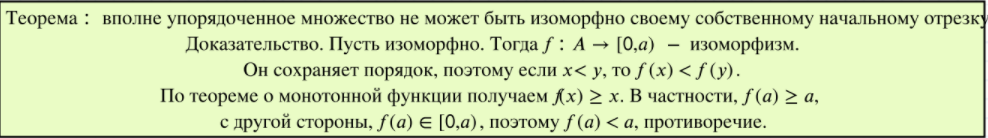
\includegraphics[width = 17cm]{images/2 (определения)_m211.PNG}
\end{center}

\subsection{Сумма и произведение фундированных множеств фундированы, вполне упорядоченных — вполне упорядочены}
Пусть сумма и произведение  фундированных множеств не фундированы. Тогда в полученном множестве существует бесконечно убывающая последовательность $(a_1, b_1) \geq (a_2, b_2) ...$, $a_1\geq a_2 ...$, из которых можно выбрать бесконечно убывающие последовательности в одном из исходных множеств, значит, оно было не фундировано

Если на множествах был линейный порядок, то в полученных множествах порядок также линеен. Так как фундированность сохраняется, полученные множества вполне упорядочены

\subsection{Свойства сложения и умножения вполне упорядоченных множеств}
\begin{itemize}
    \item [1] Ассоциативность $(\alpha + \beta) + \gamma = \alpha + (\beta + \gamma)$
    \item [2] Правая дистрибутивность $\alpha *( \beta +\gamma) = \alpha\beta + \beta \gamma$
    
\end{itemize}
    Как доказать - не нашла :(

\subsection{Сравнимость любых двух множеств по мощности (вывод из теоремы Цермело и
свойств вполне упорядоченных множеств)}
\textbf{Лемма}\\ \\
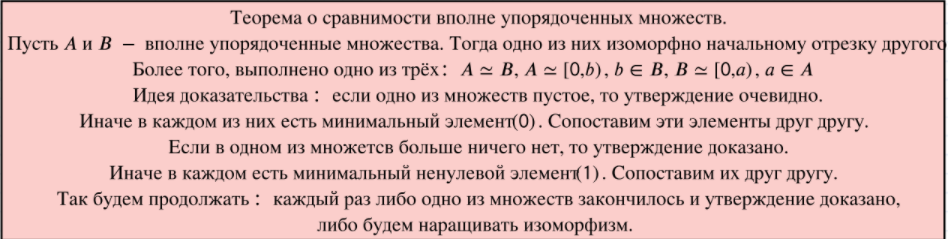
\includegraphics[width = 17cm]{images/2 (определения)_mm1.PNG}\\ \\
\textbf{Сравнимость любых двух множеств по мощности}\\
Из Теоремы Цорна мы знаем, что для любого множества существует равномощное ему ВУМ. Пусть даны $A, B$. $A', B'$ - соответственные ВУМ, удовлетворяющие теореме Цорна. Тогда из леммы следует, что эти ВУМы можно сравнить по мощности, а значит, А и В сравнимы по мощности